\section{实验报告}

\subsection{实验目的}

本实验围绕北斗/GNSS 卫星导航定位原理，完成从 RINEX 数据读取到定位结果分析的软件开发流程。实验任务包括：解析 RINEX 观测与导航文件，计算卫星位置与卫星钟差，完成传播延迟修正，利用伪距观测方程进行单点定位，并对连续历元定位结果进行精度评估和可视化展示。

完成该实验需要掌握 RINEX 数据格式、广播星历轨道计算、GPS/BDT 时间系统、ECEF 与 BLH 坐标转换、最小二乘估计、DOP 指标、对流层和电离层延迟模型，以及 Python 模块化编程、PyQt GUI 编程和 Matplotlib 可视化方法。

\subsection{实验方法和步骤}

实验采用 Python 编写完整软件系统，主要步骤如下：

\begin{enumerate}
\item 导入 RINEX 观测文件和导航文件，读取测站近似坐标、观测类型、历元数据和广播星历。
\item 对观测数据进行预处理，剔除无效伪距、不健康卫星、无星历卫星和低高度角卫星。
\item 根据广播星历计算卫星 ECEF 坐标，完成轨道摄动修正、卫星钟差修正、相对论效应修正和 TGD 改正。
\item 使用 Saastamoinen 模型进行对流层延迟改正，使用 Klobuchar 模型进行 GPS/BDS 电离层延迟改正。
\item 构建伪距定位观测方程，采用加权迭代最小二乘求解接收机位置和钟差。
\item 将 ECEF 坐标转换为经纬高坐标，计算 PDOP、GDOP、残差 RMS 和最大残差。
\item 对连续历元重复解算，输出 CSV 结果、误差统计、误差曲线、DOP 曲线、卫星数曲线和轨迹散点图。
\item 使用 GUI 验证数据导入、参数设置、实时显示、绘图和轨迹回放功能。
\end{enumerate}

\subsection{实验软件总体设计}

软件采用模块化设计，将全流程拆分为数据解析、卫星修正、定位解算、连续分析和系统界面五部分。各模块之间通过统一的数据结构传递信息，既可以通过命令行单独运行，也可以由 GUI 调用完整流程。

\begin{figure}[H]
\centering
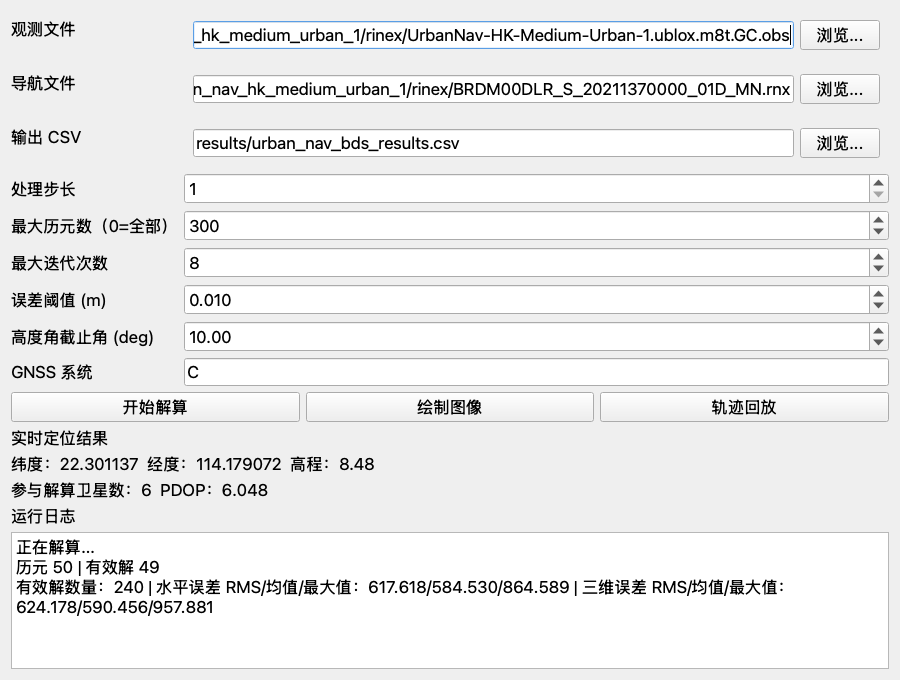
\includegraphics[width=0.82\linewidth]{figures/gui_main_window.png}
\caption{PyQt GUI 主界面}
\end{figure}

GUI 界面支持选择观测文件、导航文件和输出 CSV，设置步长、最大历元、最大迭代次数、误差阈值、高度角和 GNSS 系统。运行过程中显示最新纬度、经度、高程、使用卫星数和 PDOP；运行完成后可查看误差图并回放轨迹。

\subsection{详细设计及实现}

\subsubsection{RINEX 数据解析}

观测文件解析器支持 RINEX 2.11 与 RINEX 3。RINEX 2.11 通过 \texttt{\# / TYPES OF OBSERV} 读取观测类型；RINEX 3 通过 \texttt{SYS / \# / OBS TYPES} 分系统读取观测类型。程序按历元组织每颗卫星的观测值，保存伪距、载波相位、SNR 等信息。

导航文件解析器将广播星历保存为 \texttt{NavRecord}，包括半长轴平方根、偏心率、倾角、升交点赤经、近地点角、钟差参数、TGD 和健康状态等。对于 RINEX 3 mixed 导航文件，程序还能解析 \texttt{GPSA/GPSB/BDSA/BDSB} 电离层参数。

\subsubsection{卫星位置、钟差和传播延迟修正}

卫星位置计算基于广播星历公式。程序先计算平均角速度、平近点角、偏近点角和真近点角，再使用 \texttt{cuc/cus/crc/crs/cic/cis} 修正升交角距、轨道半径和倾角，最终转换到 ECEF 坐标系。BDS 使用 BDT 时间系统，程序在 mixed 数据中处理 GPST 到 BDT 的时间转换；BDS GEO 卫星 C01--C05 使用专门的 GEO 坐标转换分支。

卫星钟差采用钟差多项式、相对论项和 TGD 改正：

\begin{verbatim}
dt_sv = af0 + af1 * dt + af2 * dt^2 + relativistic - tgd
\end{verbatim}

传播延迟方面，对流层使用 Saastamoinen 模型，电离层使用 Klobuchar 模型。修正后的伪距进入定位方程。

\subsubsection{单点定位解算}

定位方程线性化后，采用迭代加权最小二乘求解。权重根据卫星高度角设置：

\begin{verbatim}
w = max(sin(elevation)^2, 0.05)
\end{verbatim}

GPS+BDS 联合定位时，状态向量为每个系统设置独立接收机钟差，避免 GPS 与 BDS 系统时间差被错误合并：

\begin{verbatim}
[dx, dy, dz, clock_G, clock_C]
\end{verbatim}

解算结束后输出 ECEF、BLH、接收机钟差、PDOP、GDOP、残差 RMS、最大残差和使用卫星数。

\subsubsection{连续定位、测试和可视化}

连续定位模块逐历元调用单点定位函数，并以 RINEX 头文件中的近似测站坐标作为参考，计算 ENU 方向误差、水平误差和三维误差。测试使用 UrbanNav、TWTF 等多组数据，覆盖城市动态 BDS、固定站 BDS 和 GPS+BDS 组合解算。

\begin{table}[H]
\centering
\small
\begin{tabular}{lccccc}
\toprule
数据集 & 系统 & 历元数 & 水平 RMS/m & 三维 RMS/m & PDOP 均值 \\
\midrule
UrbanNav & BDS & 240 & 617.618 & 624.178 & 6.575 \\
TWTF & BDS & 300 & 1.371 & 6.526 & 4.703 \\
TWTF & GPS+BDS & 300 & 1.208 & 2.936 & 2.755 \\
\bottomrule
\end{tabular}
\caption{重新运行后的北斗与 GPS+BDS 定位精度测试结果}
\end{table}

\begin{figure}[H]
\centering
\begin{minipage}{0.48\linewidth}
\centering

\includegraphics[width=\linewidth]{figures/urban_nav_bds_final/error_dop.png}
\caption*{(a) UrbanNav BDS 误差/DOP/卫星数曲线}
\end{minipage}
\hfill
\begin{minipage}{0.48\linewidth}
\centering
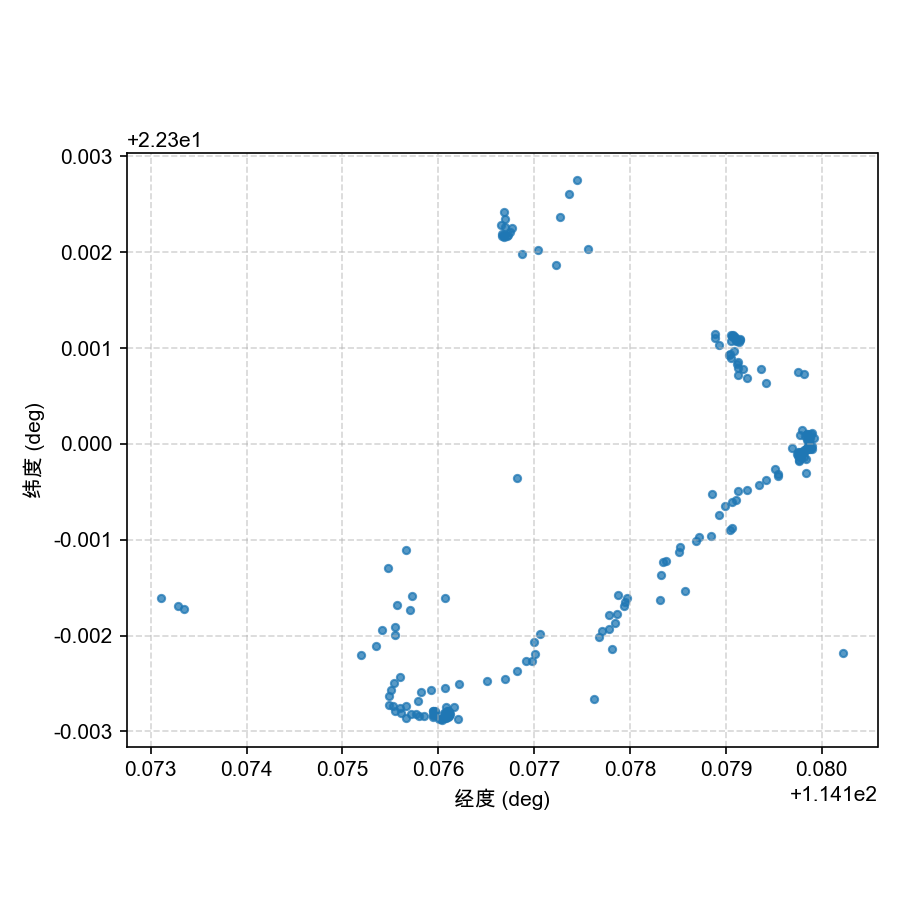
\includegraphics[width=\linewidth]{figures/urban_nav_bds_final/trajectory.png}
\caption*{(b) UrbanNav BDS 轨迹散点图}
\end{minipage}
\caption{UrbanNav 城市动态北斗定位结果}
\end{figure}

\begin{figure}[H]
\centering
\begin{minipage}{0.48\linewidth}
\centering
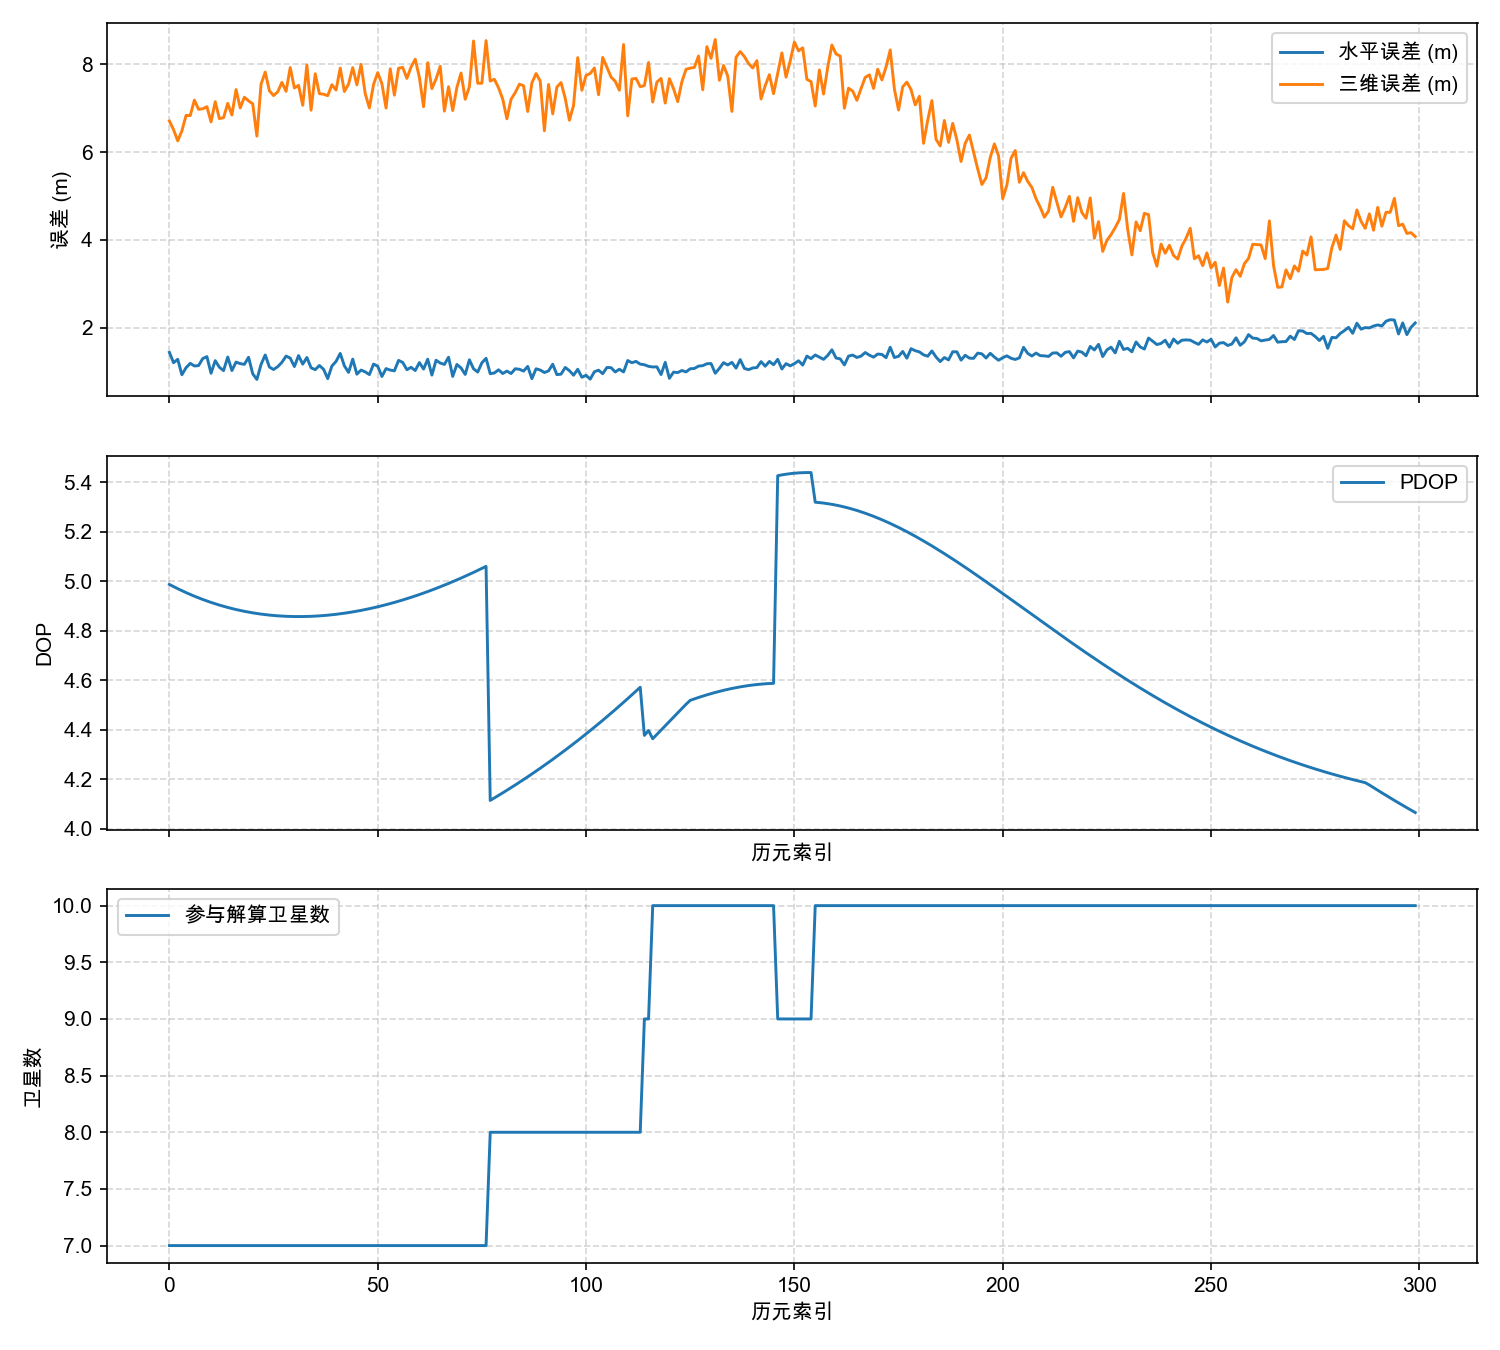
\includegraphics[width=\linewidth]{figures/twtf_bds_final/error_dop.png}
\caption*{(a) TWTF BDS-only 误差曲线}
\end{minipage}
\hfill
\begin{minipage}{0.48\linewidth}
\centering

\includegraphics[width=\linewidth]{figures/twtf_gps_bds_final/error_dop.png}
\caption*{(b) TWTF GPS+BDS 误差曲线}
\end{minipage}
\caption{TWTF 不同系统组合定位结果对比}
\end{figure}

UrbanNav 数据属于城市动态观测场景，北斗单系统定位误差明显大于固定 IGS 站数据，主要与动态接收机、多路径、遮挡和观测环境复杂有关；TWTF 固定站数据中，GPS+BDS 组合解算的 PDOP 低于 BDS-only，三维 RMS 也更小，说明多系统联合能改善卫星几何构型并提升定位稳定性。

\subsubsection{调试问题与解决}

实验过程中主要修复了以下问题：

\begin{itemize}
\item 默认数据路径与实际目录不一致，导致脚本无法开箱运行；已统一为 \texttt{data/sample/}。
\item \texttt{step=0} 会导致除零错误；已在 CLI 和 pipeline 入口增加参数校验。
\item 绘图依赖缺失时仍提示保存成功；已让绘图函数返回状态并由脚本判断。
\item BDS mixed 数据涉及 GPST/BDT 转换和 BDS 电离层参数；已解析 \texttt{BDSA/BDSB} 并修正时间转换。
\item GPS+BDS 共用单一接收机钟差会影响联合解算；已扩展为每系统独立钟差参数。
\item 对不支持的 Hatanaka \texttt{.crx/.d} 文件，程序会给出中文转换提示，避免异常退出。
\end{itemize}

\subsection{结论}

本项目完成了实验基础题要求的五个模块，能够解析 RINEX 数据、计算卫星位置与钟差、进行传播延迟修正、完成伪距单点定位和连续定位分析，并通过 GUI 展示结果。多组数据测试表明，GPS、BDS 和 GPS+BDS 均可稳定运行，能够输出定位结果、误差统计、残差诊断、CSV 文件和可视化图表。

目前系统的特点是模块边界清晰、核心算法手写、支持多系统解算和 GUI 演示。不足之处是观测权重主要基于高度角，尚未充分利用 SNR/CN0；Hatanaka 压缩文件需要外部转换后才能处理。后续可继续加入更丰富的权重模型、长期卫星残差分析和更多站点数据验证。

\subsection{结束语}

通过本次实验，我对卫星导航定位的软件实现过程有了更完整的理解。定位结果并不是单个公式直接给出，而是由数据格式解析、时间系统转换、轨道计算、误差模型和数值解算共同决定。尤其在 BDS 与 GPS mixed 数据中，时间系统、星历选择和系统钟差建模都会显著影响结果。经过多轮调试和测试，项目从单 GPS 样例扩展到 BDS-only 与 GPS+BDS 联合解算，工程可靠性和可演示性都有明显提升。

\subsection{程序清单}

\begin{verbatim}
src/
  analysis.py              误差计算与统计
  atmosphere.py            对流层与电离层改正
  constants.py             物理常数与系统常数
  coords.py                ECEF/BLH/ENU 坐标转换
  experiment_modules.py    五个实验模块封装
  gnss_systems.py          GNSS 系统参数解析与校验
  ml_compensation.py       附加题误差补偿模型
  models.py                核心数据结构
  pipeline.py              连续解算流水线与 CSV 输出
  plot_style.py            中文绘图字体配置
  plotting.py              误差曲线与轨迹散点图
  positioning.py           SPP 加权最小二乘核心
  rinex_nav.py             RINEX 导航文件解析
  rinex_obs.py             RINEX 观测文件解析
  satellite.py             广播星历卫星位置与钟差
  time_utils.py            GPS/BDT 时间工具
scripts/
  gui_app.py               PyQt GUI
  inspect_rinex.py         RINEX 文件检查
  plot_results.py          CSV 结果绘图
  run_batch.py             多数据集汇总
  run_continuous.py        连续定位 CLI
  run_spp.py               单历元定位 CLI
  train_error_model.py     附加题误差模型训练
tests/
  test_experiment_modules.py
\end{verbatim}
